\newpage

\section{Congruence via Transformations}
Informally, a \emph{transformation} of the plane is a ``motion,'' such as a rotation or a stretch of the plane, that takes a figure to an \emph{image} of that figure.  This activity explores the basic rigid motions: translations (slides), rotations (turns), and reflections (flips).  

\begin{teachingnote}
Supplies:  tracing paper.  Long rulers for drawing these on the board.  
\end{teachingnote}

\begin{prob}
One of the pairs of figures below shows a translation, and the other pair does not.  To identify which is which, draw segments between each point and its image.  Use those segments to explain your reasoning.
$$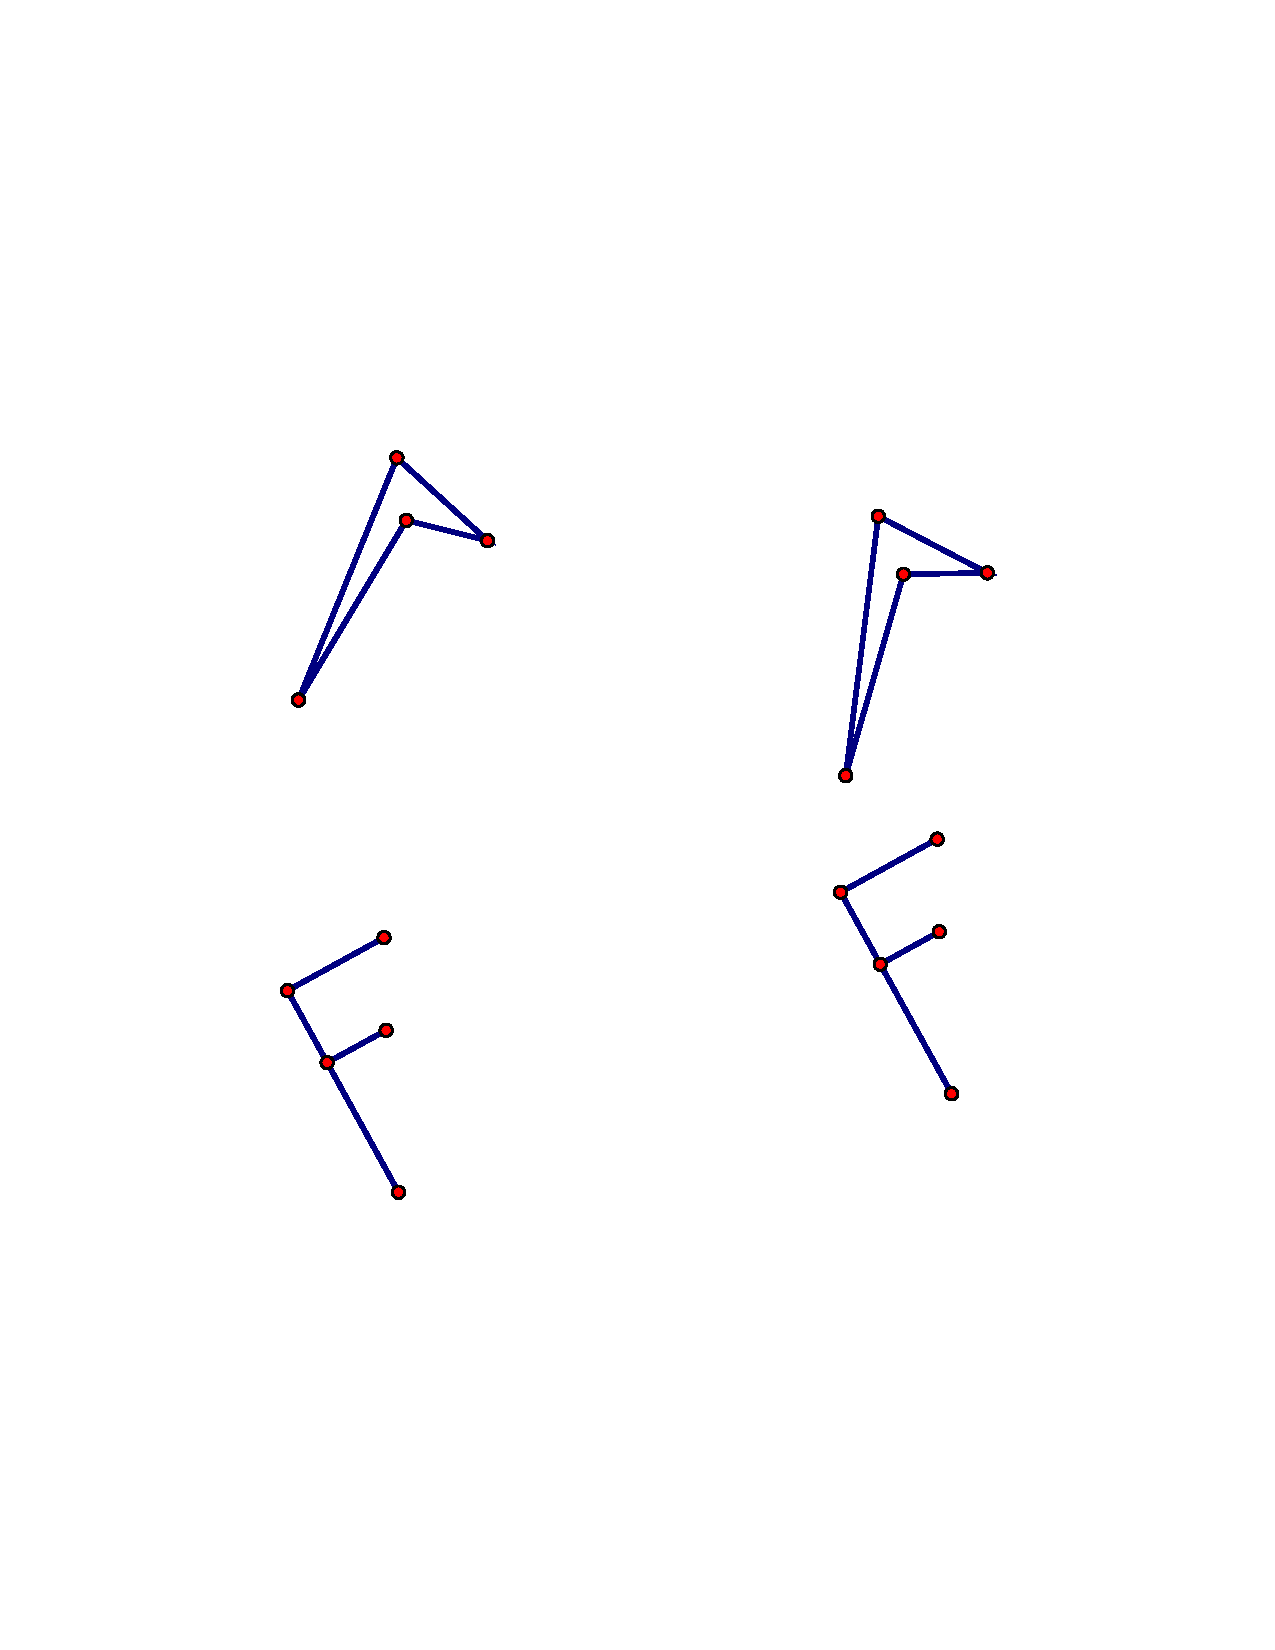
\includegraphics[scale=0.8]{../graphics/translate.pdf}$$
\end{prob}

\newpage
\begin{prob}
One of the pairs of figures shows a reflection about the given line, and the other pair does not.  
\begin{enumerate}
\item Identify which pair of figures shows a reflection about the given line, and explain how you know. 
\item Find the line of reflection for the other pair of figures, and explain your reasoning.  
$$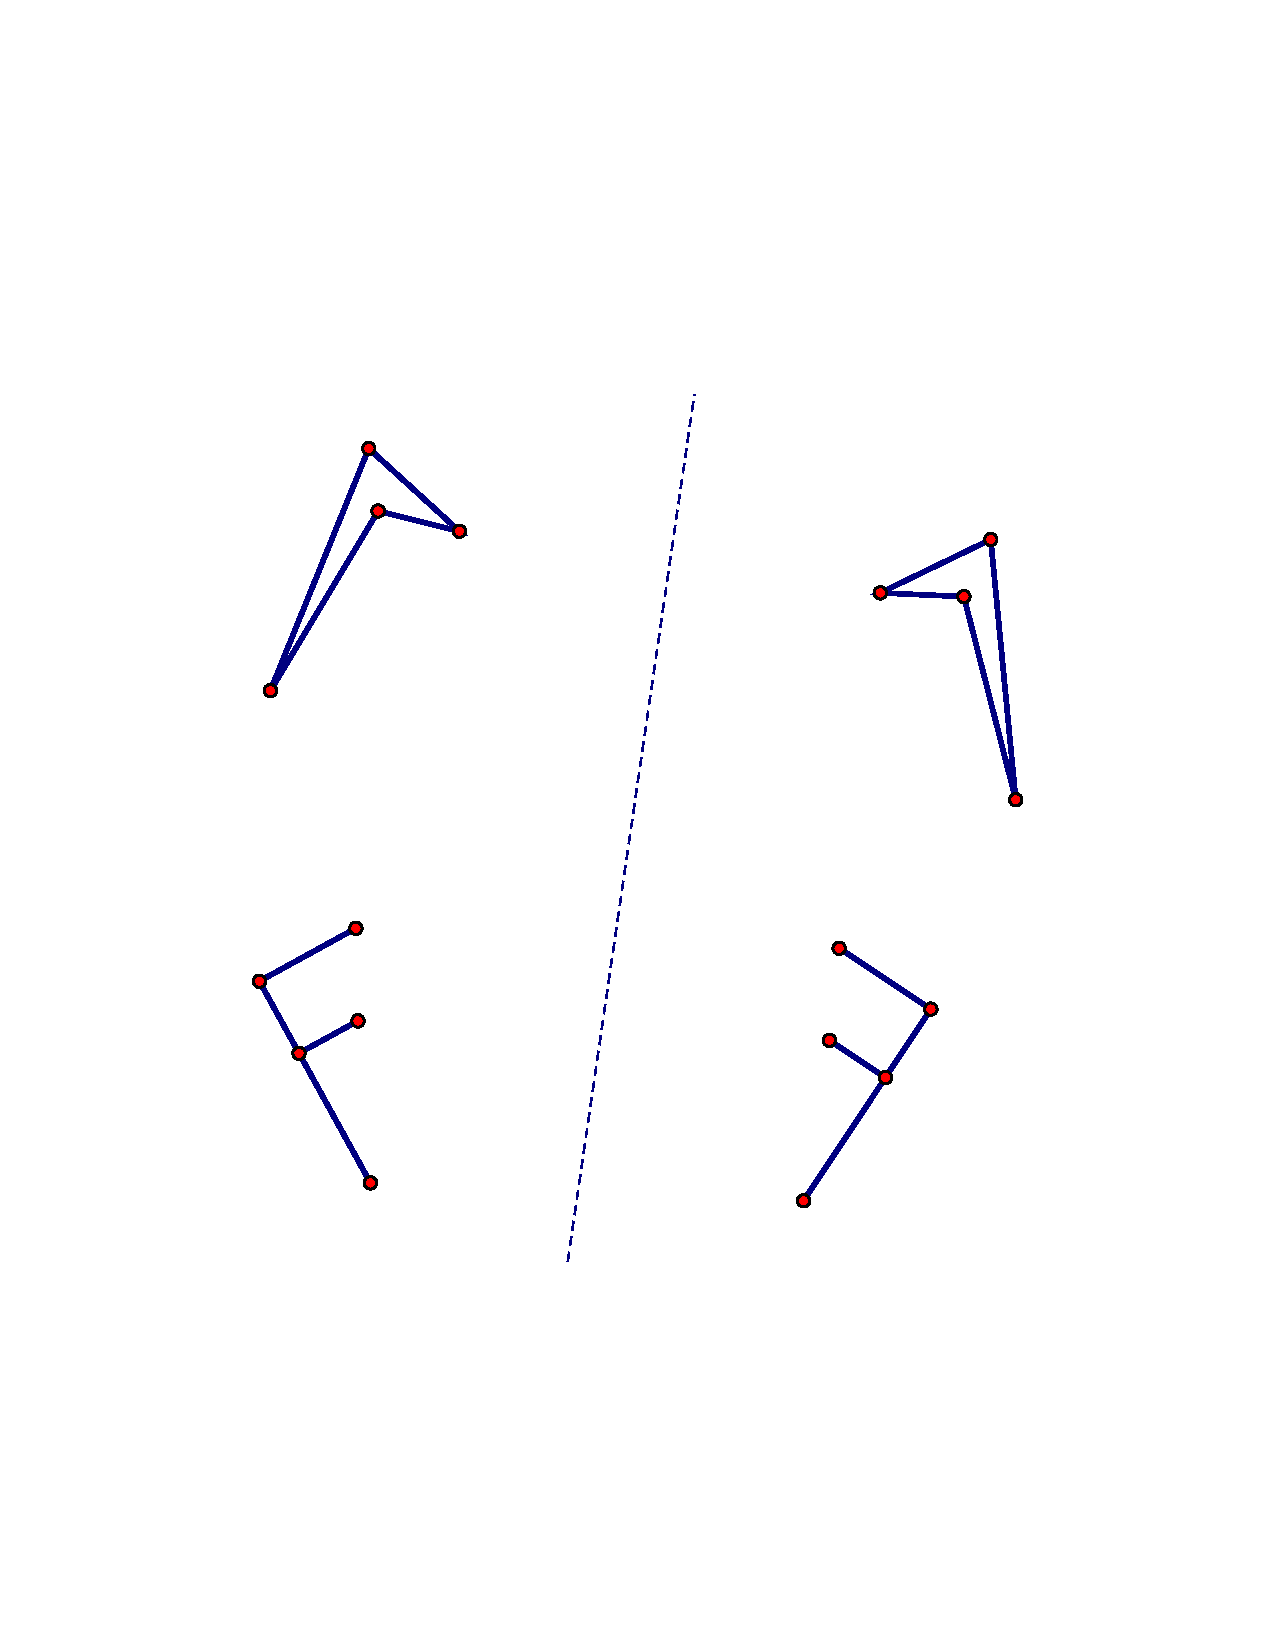
\includegraphics[scale=0.8]{../graphics/reflect.pdf}$$
\end{enumerate}
\end{prob}

\newpage
\begin{prob}
One of the pairs of figures below shows a rotation about point $C$, and the other pair does not. 
\begin{enumerate}
\item Identify which pair of figures shows a rotation about $C$, and explain how you know.  
\item Find the angle of rotation.  
\item Find the center of and angle of rotation for the other pair of figures.  Explain your reasoning.  
$$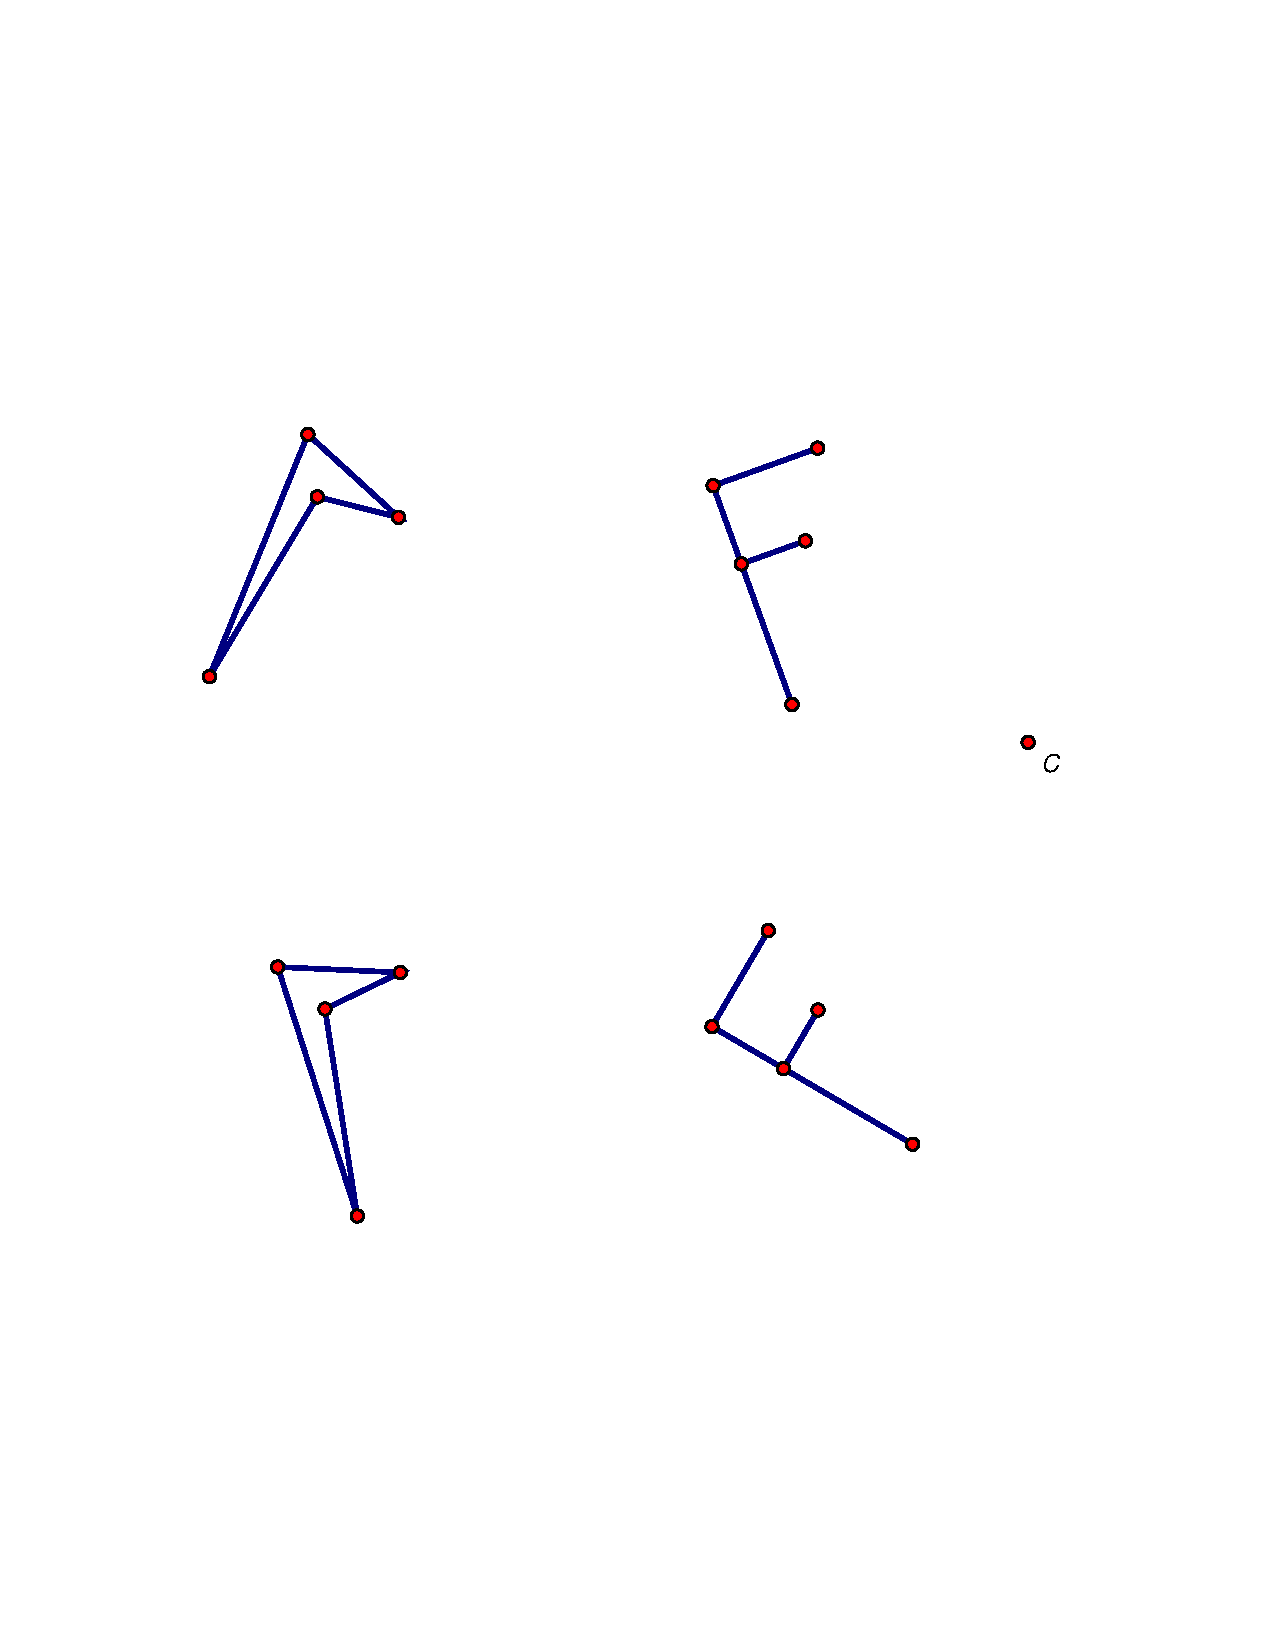
\includegraphics[scale=0.8]{../graphics/rotate.pdf}$$
\end{enumerate}
\end{prob}


\newpage
\begin{prob}
Two figures are said to be \emph{congruent} if there is a sequence of basic rigid motions that take one figure onto the other.  
\begin{enumerate}
\item Specify a sequence of two or three basic rigid motions that takes one F onto the other.  Illustrate intermediate images.  Explain your reasoning.  
\vspace{1in}
$$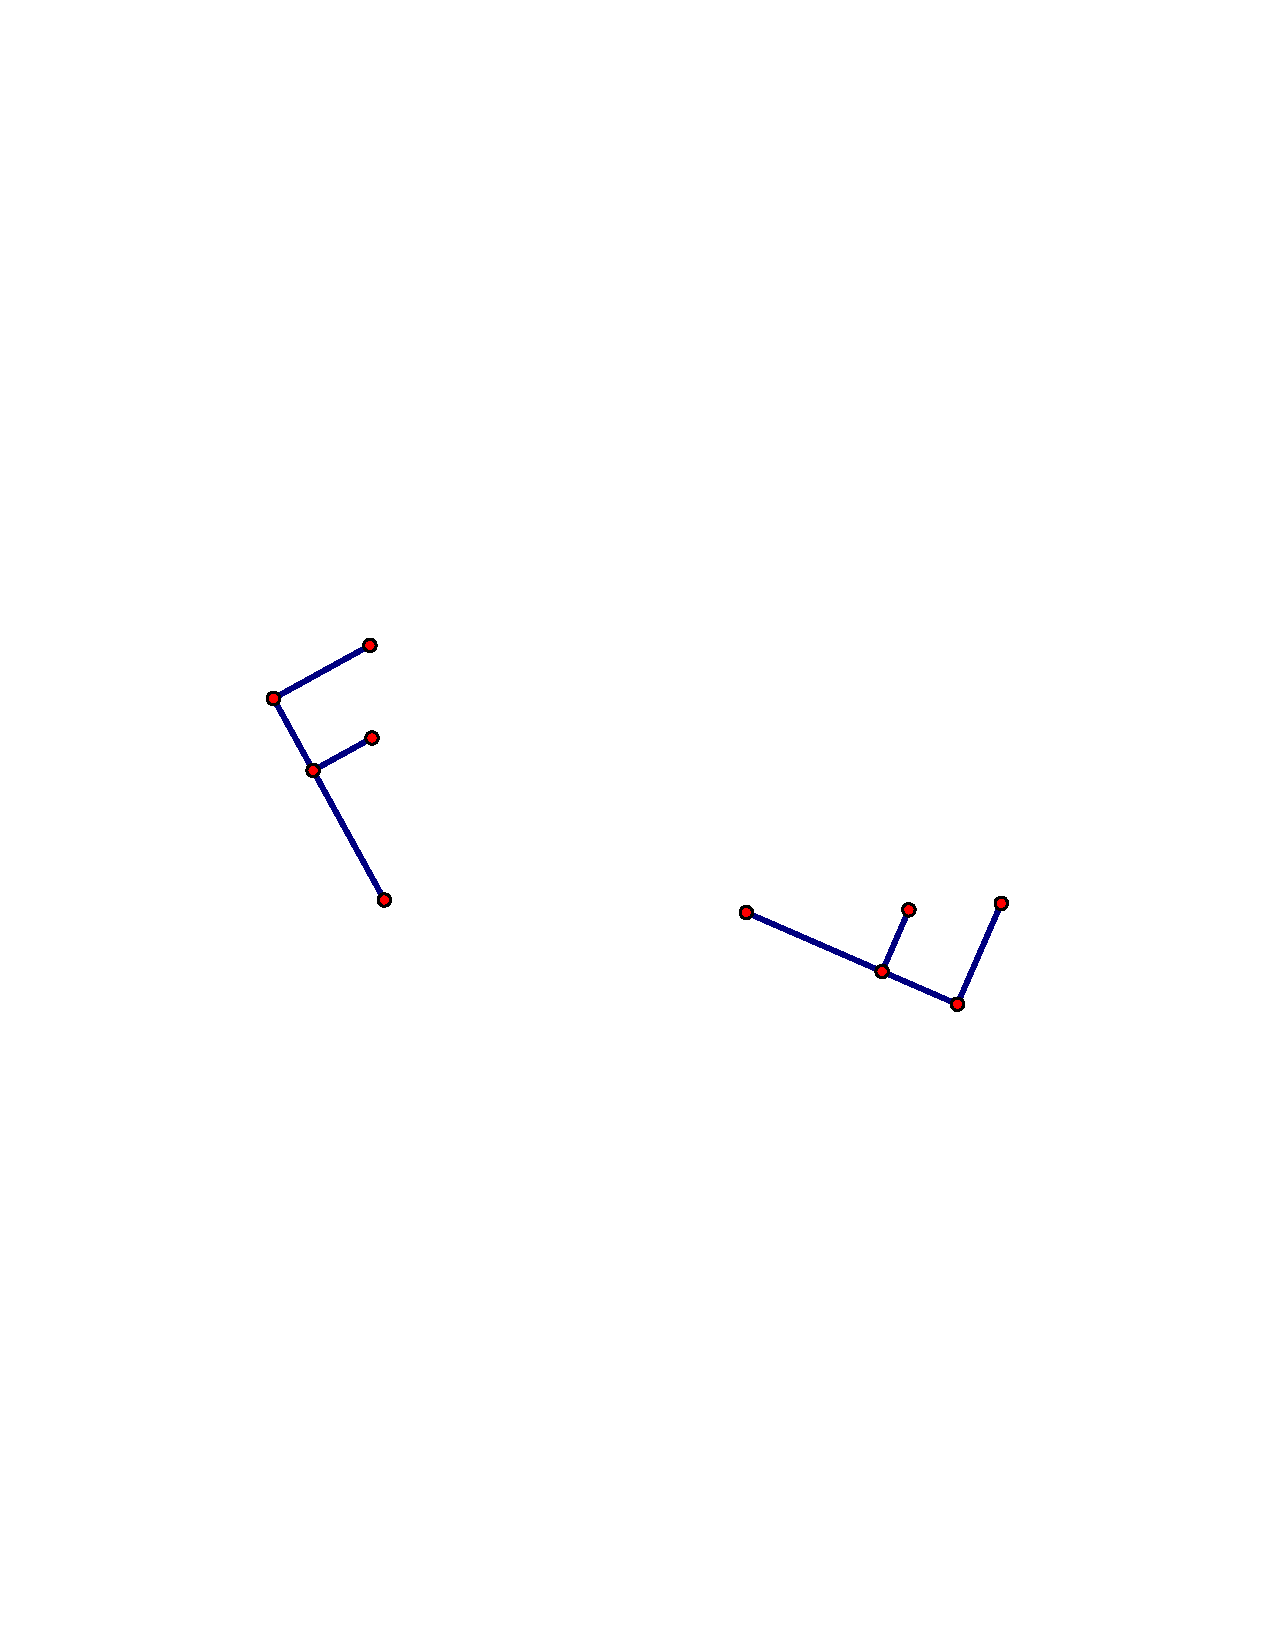
\includegraphics[scale=0.8]{../graphics/glideReflect.pdf}$$
\vspace{0.5in}
\item Explain briefly why, for this pair of figures, sequences of the following types cannot work: 
\begin{itemize}
\item a rotation followed by a rotation
\item a translation followed by a translation
\item a reflection followed by a reflection
\end{itemize}
\end{enumerate}
\end{prob}

